\documentclass{standalone}
\usepackage{amsfonts, amsmath, amssymb, bm} %Math fonts and symbols
\usepackage{dcolumn, multirow} % decimal-aligned columns, multi-row cells
\usepackage[colorlinks=true]{hyperref}
\usepackage{graphicx, subfigure, float} % graphics commands
\usepackage[margin=1in]{geometry} % sets page layout
\usepackage{setspace}% allows toggling of double/single-spacing
\usepackage{verbatim}% defines environment for un-evaluated code
\usepackage{natbib}% defines citation commands and environments.
\singlespace % set document spacing to single
\bibpunct[, ]{(}{)}{,}{a}{}{,} % sets the punctuation of the bibliography entires.
\newcolumntype{d}[1]{D{.}{.}{#1}} % defines a decimal-aligned column
\usepackage{tikz}
\usetikzlibrary{intersections}
\usepackage{enumerate}
\usepackage[utf8]{inputenc}
\usepackage[english]{babel}
\usepackage{makecell}
\usepackage{caption}
\usepackage{pgfplots}
\hyphenpenalty=10000
\definecolor{ggray}{RGB}{110,110,110}

\begin{document}
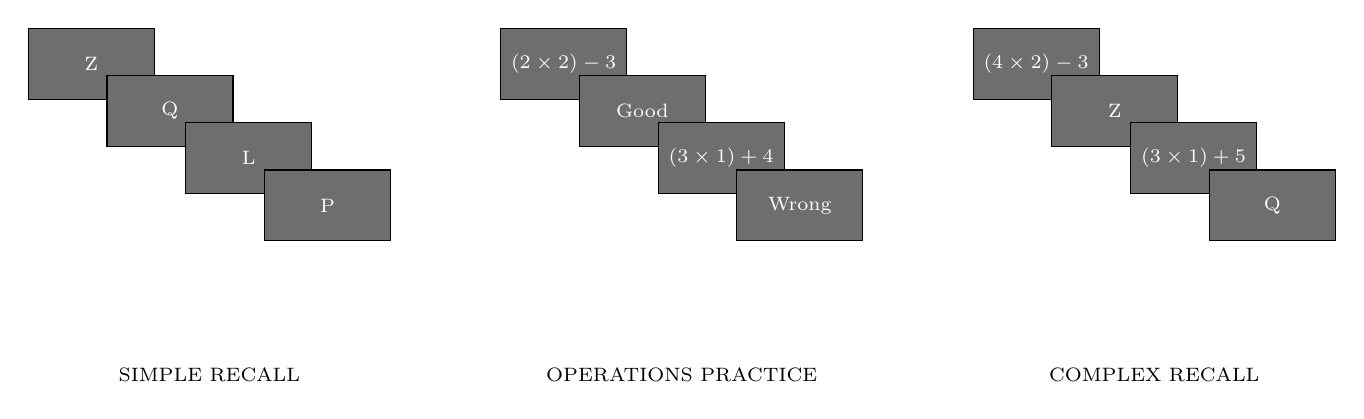
\begin{tikzpicture}[>=stealth, big/.style={scale = .5,
         % The shape:
         rectangle,
         % The size:
         minimum height=1cm,
         minimum width=2.5cm,
         % The border
         thick, draw=black,
         fill = white,
         % The filling
         % Font
         font=\itshape}]
         \begin{scope}[>=stealth]
            \foreach \x \y \w in {0/.9/Z, 1/.3/Q, 2/-.3/L, 3/-.9/P}{
            \draw [fill = ggray] (\x, \y) rectangle (\x+1.6,\y - .9);
            \draw [white] node at (\x + .8, \y - .45) {\scriptsize \w};
            };
            %% \draw [fill = ggray] (1.5,-3) rectangle (3.1, -3.9);
            %% \draw [white] node at (2.3, -3.45) {\scriptsize Recall};
            \draw node at (2.3,-3.5) {\scriptsize SIMPLE RECALL};
            \begin{scope}[xshift = 6cm]
                \foreach \x \y \w in {0/.9/$(2\times2)-3$, 1/.3/Good, 2/-.3/$(3\times1)+4$, 3/-.9/Wrong}{
                \draw [fill = ggray] (\x, \y) rectangle (\x+1.6,\y - .9);
                \draw [white] node at (\x + .8, \y - .45) {\scriptsize \w};
            };
            \draw node at (2.3,-3.5) {\scriptsize OPERATIONS PRACTICE};
            \end{scope}
            \begin{scope}[xshift = 12cm]
                \foreach \x \y \w \t in {0/.9/$(4\times2)-3$/$x + 2.5sd$, 1/.3/Z/$.8s$, 2/-.3/$(3\times1)+5$/$x + 2.5sd$, 3/-.9/Q/$.8s$}{
                \draw [fill = ggray] (\x, \y) rectangle (\x+1.6,\y - .9);
                \draw [white] node at (\x + .8, \y - .45) {\scriptsize \w};
            };
            %% \draw [fill = ggray] (1.5,-3) rectangle (3.1, -3.9);
            %% \draw [white] node at (2.3, -3.45) {\scriptsize Recall};
            \draw node at (2.3,-3.5) {\scriptsize COMPLEX RECALL};
            \end{scope}
         \end{scope}
      \end{tikzpicture}
\end{document}